\documentclass[12pt,a4paper]{article}
\usepackage[utf8]{inputenc}
\usepackage[portuguese,brazilian]{babel}
\usepackage[lmargin=3cm,tmargin=3cm,rmargin=2cm,bmargin=2cm]{geometry}
\usepackage[T1]{fontenc}
\usepackage{listings}
\usepackage{xcolor}
\usepackage{hyperref}
\usepackage{url}
\usepackage{indentfirst}
\usepackage{graphicx}
\usepackage{amsmath,amsthm,amsfonts,amssymb,dsfont,mathtools}
\usepackage{booktabs}
\usepackage{cite}
\usepackage[num]{abntex2cite}

% --- Marcador visível de pendência ---
\newcommand{\todo}[1]{\textcolor{red}{\textbf{[TODO: #1]}}}
% Caixa para figuras que ainda não existem
\newcommand{\figpendente}[1]{\fbox{\parbox{0.85\textwidth}{\centering\vspace{1.2cm}\todo{#1}\vspace{1.2cm}}}}

% --- Título e Autores ---
\title{\textbf{Modelos de decisão para testagem de casos suspeitos de arboviroses por Aprendizagem por Reforço}}

\author{
    Zuilho R. C. Segundo \quad Iasmim F. de Almeida\quad  Flávio C. Coelho  \\[0.3cm]
    \small Escola de Matemática Aplicada, Fundação Getulio Vargas (FGV EMAp) \\
    \small Rio de Janeiro, Brasil \\
}

\date{}

% --- Início do Documento ---
\begin{document}

\maketitle

\begin{abstract}
\noindent A co-circulação de dengue e chikungunya impõe um dilema recorrente à vigilância epidemiológica: o diagnóstico clínico diferencial é pouco específico, enquanto a confirmação laboratorial é escassa e cara. Este trabalho formula a alocação de exames como um processo de decisão sequencial sob incerteza, que se desenrola no tempo da própria epidemia, e avalia agentes de Aprendizagem por Reforço nesse cenário. Desenvolvemos um ambiente compatível com a interface Gymnasium em que duas epidemias coexistem: a dinâmica temporal segue um modelo SEIR com parâmetros da literatura, a distribuição espacial é estimada por \textit{Ordinary Kriging} sobre notificações reais do Rio de Janeiro (2015--2016), o diagnóstico clínico é ruidoso e os laudos laboratoriais retornam com atraso, devolvendo o caso ao agente para decisão. Mostramos que o obstáculo central do aprendizado não está na informação disponível, mas na atribuição de crédito: como os casos se sobrepõem no tempo, o valor de pedir um exame precisa atravessar dezenas de decisões sobre outros pacientes, e a estimativa de vantagem usual o apaga (correlação de $-0{,}019$ entre o retorno e o acerto do exame, contra $0{,}994$ quando o retorno é contado ao longo da linha do tempo do próprio caso). Propomos um PPO com estimativa de vantagem por caso, descontada em dias de epidemia, sem alterar o ambiente nem a recompensa. Numa primeira versão do ambiente, avaliada por bootstrap hierárquico e pareado, o crédito por caso elevou a recompensa média de $+684$ [$-146$; $+1498$] para $+2692$ [$+2523$; $+2842$] com observação idêntica e empatou estatisticamente com a melhor política fixa. Essa versão, porém, não continha casos de outras etiologias, o que tornava um único exame sempre suficiente. No ambiente corrigido, em que um laudo negativo deixa de resolver o caso, o agente com crédito por caso \emph{supera} a melhor política fixa (testar os dois vírus em todos os casos) em $+1163$ [$+980$; $+1330$] pontos, vencendo-a em todos os 10 cenários pareados, com a mesma acurácia (0,938) e 31\% menos exames: aprende quais casos precisam do segundo exame. O agente com a estimativa de vantagem usual colapsa para a inação, abaixo da própria triagem clínica. Esses resultados no ambiente corrigido são preliminares, com uma única semente de treino por braço.

\noindent \textbf{Palavras-chave:} Aprendizagem por Reforço. Arboviroses. Modelos de Decisão. Alocação de Recursos. Vigilância Epidemiológica.
\end{abstract}

% =====================================================================
\section{Introdução}
% =====================================================================

As arboviroses estão entre os desafios mais complexos e persistentes da saúde pública global, impondo uma carga epidemiológica severa, sobretudo em regiões tropicais e subtropicais como o Brasil \cite{govbr_arboviroses}. Doenças como dengue, chikungunya e Zika, que compartilham o vetor \textit{Aedes aegypti}, manifestam-se em epidemias cíclicas de grande escala que periodicamente sobrecarregam os sistemas de saúde. Esses surtos geram impactos socioeconômicos profundos, que vão da perda de produtividade do trabalho ao aumento expressivo dos custos diretos de internação e atendimento de urgência \cite{donateli_visualizacao_2023, ministério2024boletim}. A co-circulação simultânea desses vírus agrava o cenário epidemiológico, criando uma sobreposição de quadros clínicos que dificulta a vigilância em tempo real e exige respostas rápidas e coordenadas. A dengue, em particular, permanece uma ameaça endêmica e epidêmica, que demanda investimentos contínuos em controle vetorial e manejo clínico preventivo para mitigar a morbimortalidade associada às formas graves \cite{junior_epidemiology_2022}.

Um obstáculo crítico no manejo dessas epidemias está na dificuldade intrínseca do diagnóstico clínico diferencial, agravada pela escassez de recursos para confirmação laboratorial em massa. A definição de caso suspeito recomendada pelo Ministério da Saúde, tipicamente baseada em febre súbita associada a artralgia, mialgia ou exantema, tem alta sensibilidade para captar indivíduos infectados, mas baixa especificidade para distinguir a etiologia viral \cite{govbr_chick}. Em cenários de transmissão simultânea, diferenciar dengue de chikungunya apenas pela anamnese e pelo exame físico torna-se uma tarefa sujeita a muitos erros \cite{arrubla-hoyos_methodology_2024}. Esses fatores resultam com frequência em subnotificação ou classificação incorreta, o que compromete a compreensão da dinâmica de transmissão e a formulação de políticas públicas. Além disso, em surtos de rápida expansão, a confirmação laboratorial universal --- adotada neste estudo como padrão-ouro diagnóstico --- torna-se financeira e logisticamente inviável, obrigando os gestores a restringir o uso de exames. Muitas vezes essa priorização ocorre de forma reativa e ineficiente: insumos valiosos são gastos em casos clinicamente evidentes, enquanto casos atípicos ou epidemiologicamente estratégicos permanecem sem confirmação \cite{junior_epidemiology_2022}.

Consequentemente, a alocação de exames laboratoriais transcende a esfera puramente clínica e constitui um problema de decisão sequencial sob incerteza. A escolha de testar um caso suspeito, apoiar-se no vínculo epidemiológico, aguardar informação adicional ou atribuir um diagnóstico final não é um evento isolado: consome recursos finitos e afeta a qualidade da vigilância futura \cite{yu_deep_2023}. Embora as abordagens anteriores tenham se concentrado sobretudo na classificação de casos ou na previsão de surtos, poucos estudos trataram a alocação de exames como um problema de decisão sequencial sob incerteza epidemiológica. Esse cenário pode ser formalizado como um problema de otimização estocástica e controle dinâmico, no qual o agente decisor precisa equilibrar o custo logístico imediato de testar contra o risco latente de um diagnóstico incorreto e de uma resposta tardia de saúde pública \cite{yaesoubi_generalized_2011}. Além disso, como o estado verdadeiro da epidemia é apenas parcialmente observável --- por atrasos de notificação, incerteza clínica e infecções assintomáticas ---, políticas dinâmicas de saúde exigem modelos capazes de raciocinar a partir de informação incompleta e de atualizar decisões ao longo do tempo \cite{yaesoubi_generalized_2011,sutton2018reinforcement}.

Para enfrentar essa lacuna, este trabalho desenvolve e avalia agentes de Aprendizagem por Reforço Profundo (\textit{Deep Reinforcement Learning}, DRL) para otimizar políticas de alocação de exames em casos suspeitos de arboviroses. Diferentemente de modelos preditivos estáticos, voltados apenas à classificação, a hipótese central é que um agente computacional, treinado num ambiente de simulação epidemiológica compatível com a interface Gymnasium \cite{noauthor_gymnasium_nodate, lapan2020deep}, pode aprender autonomamente políticas dinâmicas de testagem --- decidindo não apenas \emph{quanto} investigar, mas \emph{quem} investigar. A formulação preserva deliberadamente a dinâmica temporal da epidemia: as decisões acontecem dia a dia, dentro do tempo epidêmico, com casos que chegam, aguardam laudos e voltam ao agente. Essa escolha tem um preço, que acabou se revelando o ponto central do trabalho: como muitos casos estão abertos ao mesmo tempo, as consequências de uma decisão sobre um paciente chegam intercaladas com as de dezenas de outros, e os algoritmos usuais de Aprendizagem por Reforço não conseguem atribuir a cada decisão o crédito que lhe cabe.

As contribuições deste trabalho são quatro: (i) a formalização do diagnóstico diferencial espacializado como processo de decisão sequencial no tempo da epidemia, num ambiente que combina um modelo SEIR com parâmetros de literatura e uma distribuição espacial estimada a partir de notificações reais; (ii) o diagnóstico, com uma medição direta, de que o gargalo do aprendizado é a atribuição de crédito entre casos intercalados, e não a informação disponível ao agente; (iii) um PPO com estimativa de vantagem por caso, descontada em dias de epidemia, que mantém inalterados o ambiente e a recompensa; e (iv) um protocolo de avaliação com comparações pareadas e bootstrap hierárquico, que declara as fontes de variância. As políticas aprendidas são comparadas com políticas fixas triviais que estabelecem piso e teto de desempenho, sem as quais um agente pode parecer competente apenas por ser melhor que o acaso.

% =====================================================================
\section{Metodologia}
% =====================================================================

\subsection{Desenho do estudo}

Este estudo avalia algoritmos de Aprendizagem por Reforço como suporte à decisão diagnóstica e à alocação de exames em casos suspeitos de arboviroses por meio de experimentos computacionais (Figura \ref{fig:fluxograma_metodos}). O arcabouço foi organizado em quatro fases. Primeiro, um modelo de simulação estocástica gera surtos simultâneos de dengue e chikungunya, com dinâmica temporal SEIR e distribuição espacial sintética ou estimada por \textit{kriging} sobre dados reais. Segundo, esse cenário é formulado como um Processo de Decisão de Markov (MDP) em tempo discreto, no qual as decisões de diagnóstico e testagem são ações sequenciais sob incerteza \cite{sutton2018reinforcement}. Terceiro, implementamos e treinamos agentes que vão de políticas fixas simples a métodos de Aprendizagem por Reforço Profundo, incluindo a variante com atribuição de crédito por caso proposta aqui. Por fim, avaliamos cada agente por recompensa acumulada, acurácia diagnóstica e número de exames solicitados, com comparações pareadas por cenário e intervalos de confiança por bootstrap hierárquico.

\begin{figure}[htbp]
    \centering
    \figpendente{fluxograma do desenho experimental: geração de surtos (SEIR + kriging), formulação do MDP, treino dos agentes e avaliação pareada com bootstrap}
    \caption{Fluxograma do desenho experimental, da geração dos dados simulados ao treinamento e à avaliação dos agentes de Aprendizagem por Reforço.}
    \label{fig:fluxograma_metodos}
\end{figure}

\subsection{Dinâmica temporal: modelo SEIR}
\label{subsec:seir}

A dinâmica temporal de cada doença é gerada por um modelo compartimental SEIR (Suscetível, Exposto, Infeccioso, Recuperado) em população fechada, com transmissão dependente de frequência \cite{side2015sir, derouich_model_2003}:
\begin{equation}
\begin{gathered}
    \dot S = -\beta \frac{S I}{N}, \qquad
    \dot E = \beta \frac{S I}{N} - \sigma E, \\
    \dot I = \sigma E - \gamma I, \qquad
    \dot R = \gamma I,
\end{gathered}
    \label{eq:seir}
\end{equation}
com $\sigma = 1/\text{latência}$, $\gamma = 1/\text{período infeccioso}$ e $\beta = R_0\,\gamma$. A notificação acompanha o fluxo $\sigma E$, isto é, o início da fase infecciosa, que aproximamos pelo início dos sintomas. O sistema é integrado numericamente para obter a curva acumulada de notificações $C(t)$, e os casos novos de cada dia são $N_{d}(t) = \text{round}(C_{d}(t) - C_{d}(t-1))$.

Dengue e chikungunya são transmitidas pelo \textit{Aedes}, e o intervalo entre casos sucessivos inclui o ciclo no mosquito. Em vez de um modelo hospedeiro--vetor completo, adotamos um período latente humano \emph{efetivo}, que absorve as incubações intrínseca e extrínseca, de modo que o tempo de geração do modelo (latência mais período infeccioso) corresponda ao intervalo serial observado em campo. Isso preserva o \emph{tempo} da epidemia --- o que o ambiente precisa --- com dois parâmetros por doença (Tabela \ref{tab:seir}). Para a dengue, a incubação intrínseca tem média de 5,9 dias \cite{chan2012incubation}, a infecciosidade humana dura cerca de cinco dias após o início dos sintomas \cite{carrington2014human}, e o agrupamento espaço-temporal mais forte ocorre no intervalo de 15 a 17 dias \cite{aldstadt2012spacetime}; o $R_0$ estimado para o Rio de Janeiro foi de 1,70 em 2002 e 1,25 em 2012 \cite{villela2017zika}. Para a chikungunya no Rio, estimou-se $R_0 = 1{,}56$ (IC 95\%: 1,46--1,67), assumindo tempo de geração de 14 dias \cite{moreira2023chikungunya}; a divisão entre latência e período infeccioso não tem fonte direta, e só a soma está ancorada.

\begin{table}[htbp]
\centering
\begin{tabular}{lcccc}
\toprule
\textbf{Doença} & \textbf{Latência efetiva} & \textbf{P. infeccioso} & \textbf{T. de geração} & $\boldsymbol{R_0}$ \\ \midrule
Dengue & 11 d & 5 d & 16 d & 1,25--1,70 \\
Chikungunya & 8 d & 6 d & 14 d & 1,46--1,67 \\ \bottomrule
\end{tabular}
\caption{Parâmetros do modelo SEIR. A cada episódio, o $R_0$ de cada doença é sorteado uniformemente na faixa indicada. Fontes: \citeonline{chan2012incubation, carrington2014human, aldstadt2012spacetime, villela2017zika, moreira2023chikungunya}.}
\label{tab:seir}
\end{table}

Cada episódio cobre 300 dias epidemiológicos, com população de 300 indivíduos por doença e 1\% de infectados iniciais repartidos entre $E$ e $I$ na proporção das durações --- a dengue é endêmica no Rio, e uma temporada não começa de um único caso importado. Com esses valores, 95\% dos casos ocorrem entre os dias 159 e 302 em toda a faixa de $R_0$, e cada doença atinge a fração prevista pela equação do tamanho final $z = 1 - e^{-R_0 z}$ (37--69\% na dengue, 56--68\% na chikungunya). Uma consequência da literatura merece registro: o $R_0$ da chikungunya no Rio é comparável ao da dengue, e não sistematicamente menor. Versões anteriores do ambiente tratavam a chikungunya como surto secundário sempre menor, o que era escolha de desenho, não achado epidemiológico. \todo{confirmar com o orientador a premissa de $R_0$ da chikungunya, cujas faixas de literatura se sobrepõem às da dengue}

A escolha do modelo não é um detalhe. A primeira versão do ambiente usava um SIR cuja força de infecção não era dividida pela população e cujo período infeccioso era de 250 dias: um $R_0$ declarado de 1,5 valia, na prática, 225, e a epidemia inteira cabia em nove dias, com pico no terceiro (Figura \ref{fig:seir}). As curvas tinham formato plausível --- só a epidemiologia estava errada ---, e toda a estrutura temporal do ambiente, da sobreposição de casos à espera pelo laudo, estava calibrada a esse pico artificial. Com o SEIR, o número de dias com notificação passou de 9 para 184, o pico de 60 para 4 casos por dia, e o intervalo entre duas decisões sobre o mesmo caso de 278 para cerca de 30 passos. Por isso a validação do gerador verifica propriedades conferíveis contra a teoria --- o $R_0$ efetivo medido pela taxa de crescimento (dentro de 3\% do declarado), a equação do tamanho final e a duração em meses ---, e não o formato das curvas.

\begin{figure}[htbp]
\centering
\includegraphics[width=\textwidth]{../results/demo/modelo_seir.png}
\caption{Dinâmica temporal do ambiente. À esquerda, incidência diária gerada pelo SEIR para dengue e chikungunya, comparada com o modelo SIR original, cuja epidemia se esgotava em poucos dias. À direita, fração final infectada produzida pelo gerador em função do $R_0$, sobreposta à equação do tamanho final.}
\label{fig:seir}
\end{figure}

\subsection{Distribuição espacial dos casos}
\label{subsec:espacial}

Os casos de cada dia são posicionados numa grade bidimensional de $400 \times 400$ células por um gerador intercambiável, o que permite contrastar uma geometria idealizada com uma distribuição urbana empírica mantendo todos os demais parâmetros fixos.

\paragraph{Gerador sintético.} As posições são amostradas de normais bivariadas truncadas em torno de um epicentro $(\mu_x, \mu_y)$ por doença, com dispersão $\sigma$ (Figura \ref{fig:distribuicao_casos}):
\begin{align*}
c_x &\sim \mathcal{N}_{T}(\mu_{x,d}, \sigma_{d}^2;\, 0, L-1), &
c_y &\sim \mathcal{N}_{T}(\mu_{y,d}, \sigma_{d}^2;\, 0, L-1).
\end{align*}
Os dois focos são limpos e bem separados; medido empiricamente, a posição do caso, sozinha, acerta a doença em 93,7\% das vezes.

\begin{figure}[htbp]
\centering
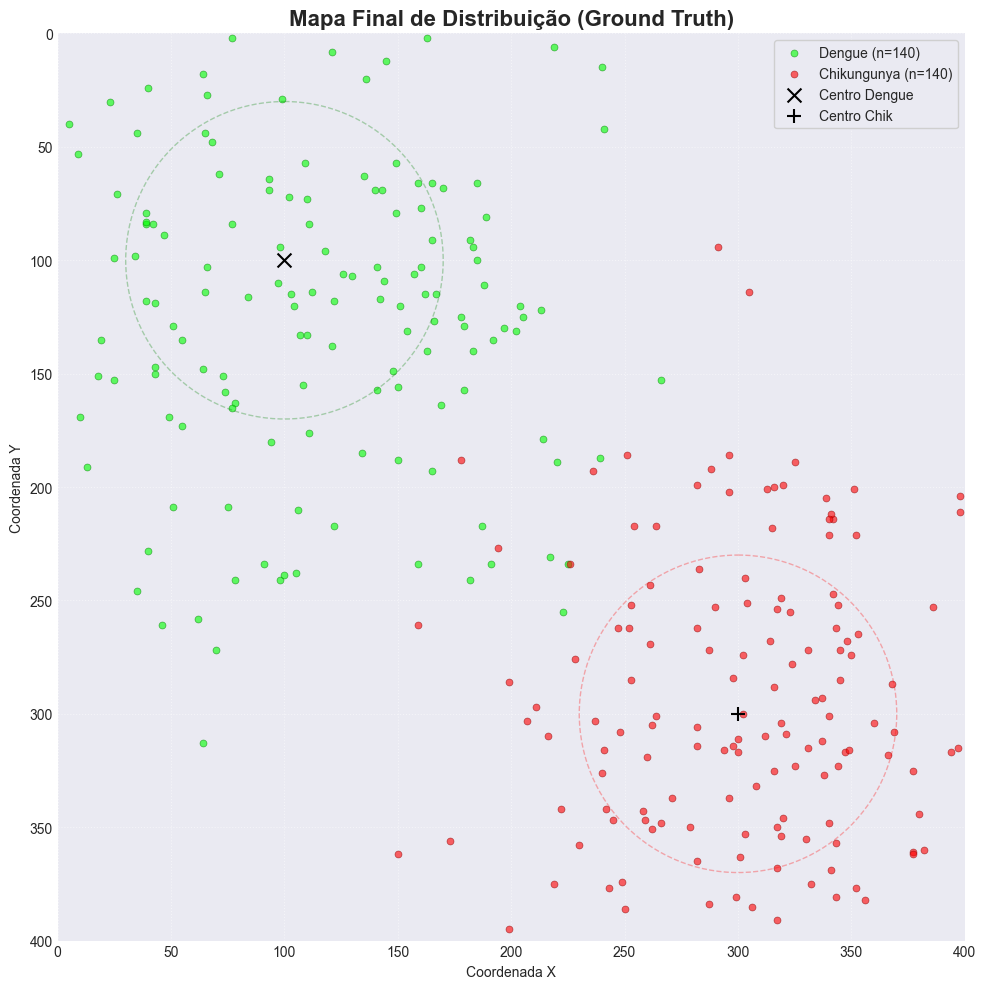
\includegraphics[width=0.5\linewidth]{img/casos.png}
\caption{Exemplo da distribuição espacial dos casos no gerador sintético, na grade $400 \times 400$, com a sobreposição entre dengue (verde) e chikungunya (vermelho).}
\label{fig:distribuicao_casos}
\end{figure}

\paragraph{Gerador por \textit{kriging}.} O ambiente de referência usa superfícies estimadas por \textit{Ordinary Kriging} sobre as notificações de dengue e chikungunya do Rio de Janeiro em 2015--2016. As superfícies interpoladas são normalizadas numa probabilidade espacial por doença, $P(\text{célula} \mid \text{doença})$, da qual os casos são amostrados (Figura \ref{fig:kriging}). A Zika fica de fora, pois o ambiente modela apenas dengue e chikungunya. A cada episódio, uma de quatro transformações rígidas (identidade, rotação de $180^\circ$, espelhamento horizontal ou vertical) é aplicada \emph{conjuntamente} às duas superfícies, para que o agente não decore a geografia de um único surto: a transformação muda \emph{onde} estão os focos, mas preserva a geometria relativa entre as doenças e, portanto, a dificuldade.

A diferença entre os dois geradores é o que torna o cenário real interessante. Cada superfície do \textit{kriging}, isoladamente, tem focos nítidos; o que importa, porém, é a razão entre elas, e os focos das duas doenças coincidem. As superfícies de dengue e chikungunya têm correlação de 0,85 --- ambas seguem onde as pessoas moram e onde está o vetor --- e, em 90\% das células, uma doença é no máximo cerca de 1,4 vez mais provável que a outra (a razão entre elas vai de 0,68 a 1,42, com extremo de 2 em todo o mapa). O melhor classificador que vê apenas a posição (acurácia de Bayes, com prior igual entre as doenças) acerta 54,4\%, pouco acima do acaso. No sintético a geografia praticamente resolve o problema; no cenário real, o exame passa a ser a principal fonte de informação.

\begin{figure}[htbp]
\centering
\includegraphics[width=\textwidth]{../results/demo/kriging.png}
\caption{Superfícies de probabilidade espacial estimadas por \textit{kriging} sobre as notificações do Rio de Janeiro: $P(\text{célula} \mid \text{dengue})$, $P(\text{célula} \mid \text{chikungunya})$ e o contraste entre elas. O contraste fraco é o que faz a posição do caso, sozinha, pouco informar sobre a doença.}
\label{fig:kriging}
\end{figure}

\paragraph{Variações do cenário real.} Para testar a robustez das conclusões à geografia, o gerador aceita duas famílias de variação. A primeira troca o ano das notificações: como a chikungunya quase não circulou no Rio em 2015 (70 notificações, contra cerca de 14 mil em 2016), uma superfície de chikungunya de 2015 não é estimável, e os cenários alternativos são ``dengue 2015 com chikungunya 2016'' e ``Rio 2016''. A segunda controla \emph{quanto} a posição informa a doença, preservando onde estão os focos: uma temperatura $\tau$ reescala as superfícies ($p \propto p^{\tau}$; $\tau=0$ é a uniforme e $\tau>1$ concentra a massa nos focos), e há ainda corte por quantis e mistura com a uniforme. A acurácia de Bayes da posição vai de 0,50 em $\tau=0$ a 0,94 em $\tau=32$, o nível de separação do gerador sintético. A temperatura alcança essa separação concentrando cada doença nos seus focos, o que tem limite de plausibilidade: metade dos casos de dengue cai em 34\% das células em $\tau=1$, em 1\% em $\tau=8$ e em apenas 8 das 13.195 células em $\tau=32$ (Figura \ref{fig:razao}). Os valores intermediários ($2 \le \tau \le 8$) preservam o desenho dos focos; $\tau=32$ é um extremo artificial, útil como limite, mas não como epidemia plausível.

\begin{figure}[htbp]
\centering
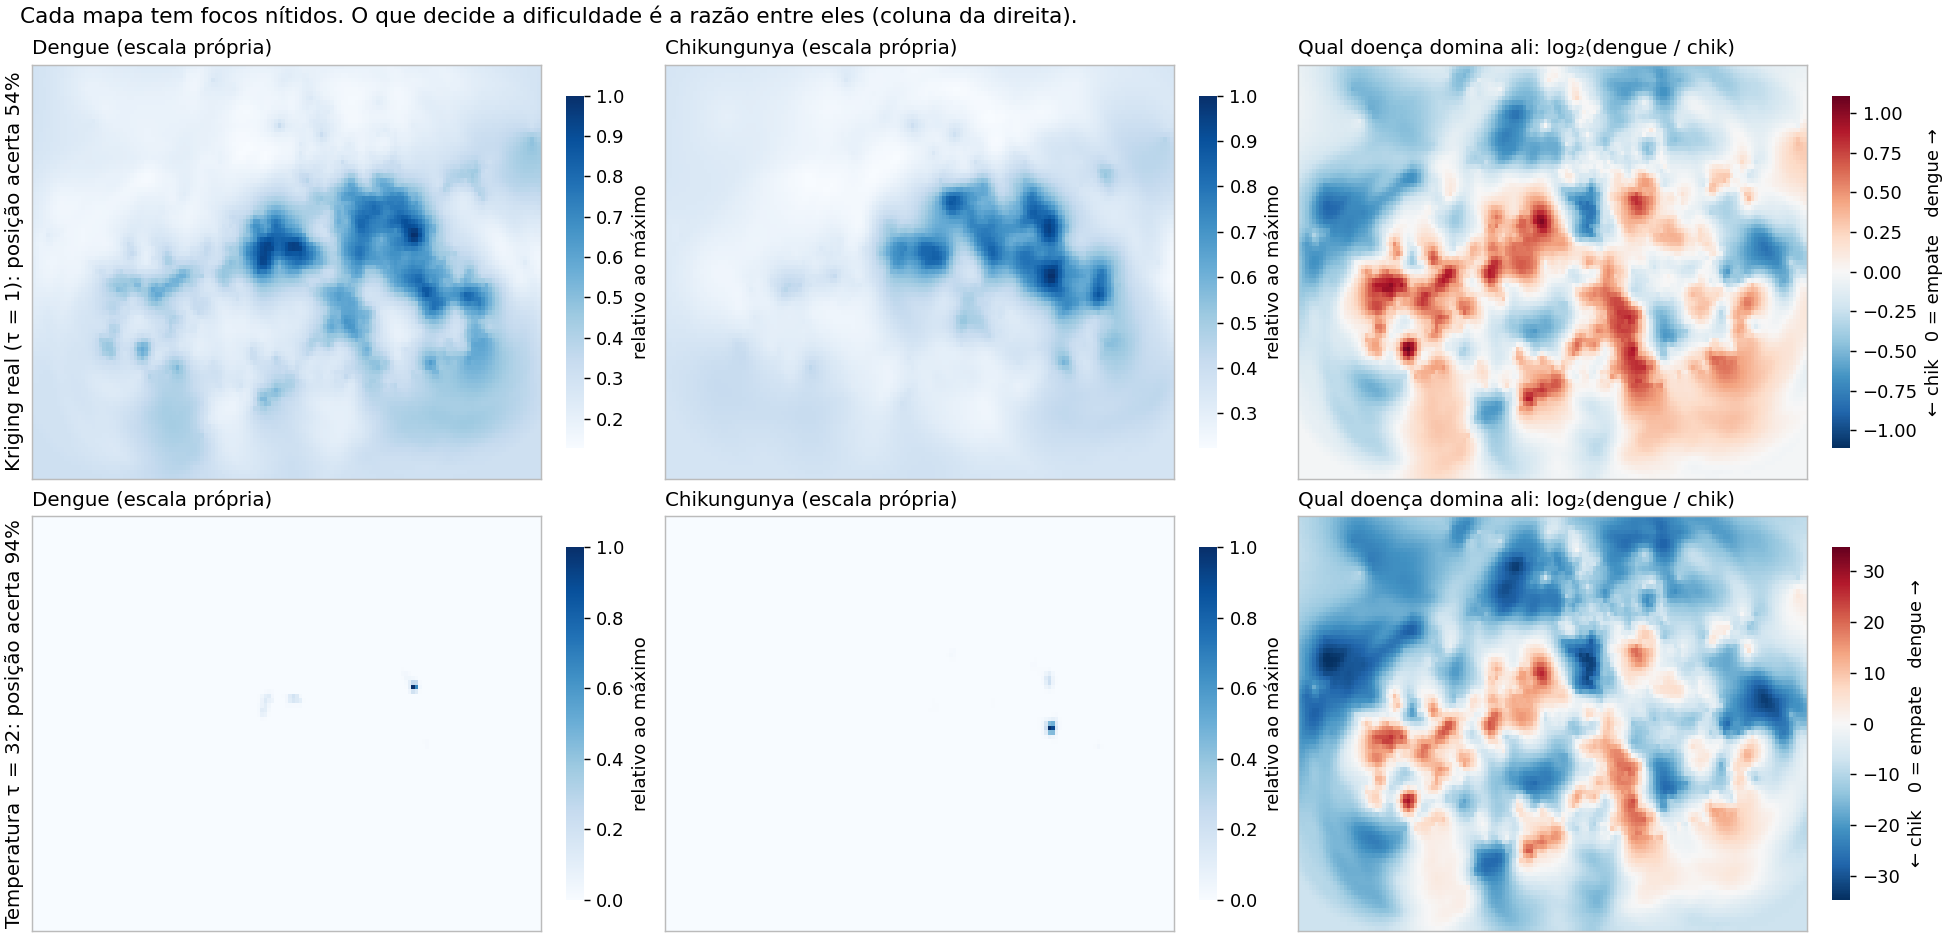
\includegraphics[width=\textwidth]{img/superficies_razao.png}
\caption{Superfícies de dengue e chikungunya, cada uma na própria escala, e a razão entre elas, $\log_2(\text{dengue}/\text{chik})$. Em cima, o \textit{kriging} real ($\tau=1$): focos nítidos em cada doença, mas razão entre $0{,}5\times$ e $2\times$, e a posição acerta a doença em 54\%. Embaixo, $\tau=32$: a razão fica enorme (acerto de 94\%), mas cada doença colapsa em poucas células.}
\label{fig:razao}
\end{figure}

\paragraph{Casos que não são arboviroses.} Na triagem real, boa parte dos casos suspeitos não se confirma. O gerador sintético produz, além de dengue e chikungunya, síndromes febris de outra etiologia, com prevalência de 25\% dos casos notificados, uniformes no espaço (não seguem os focos do vetor) e em número proporcional aos casos arbovirais de cada dia. É a presença desses casos que dá profundidade à investigação: um laudo negativo de dengue deixa de implicar chikungunya, e concluir ``não é arbovirose'' passa a ser uma decisão legítima. Como discutido na Seção \ref{subsec:ressalva}, o gerador por \textit{kriging} ignorava esse parâmetro na primeira versão do ambiente de referência (v8). Na versão corrigida (v9), idêntica ao v8 em todo o resto, o gerador por \textit{kriging} passa a produzir esses casos pelo mesmo modelo do sintético, e eles somam cerca de um quarto dos casos notificados (por exemplo, o cenário de semente 100 tem 180 casos de dengue, 180 de chikungunya e 123 de outra etiologia).

\subsection{Incerteza clínica: modelando o médico}
\label{subsec:clinico}

Para simular a incerteza da triagem real, a doença verdadeira de cada indivíduo é ocultada do agente e substituída por uma classificação clínica preliminar ruidosa. Tomando a dengue como classe positiva, essa classificação é governada por dois parâmetros do médico que atende o caso:
\begin{align*}
\text{sensibilidade} &= P(\text{rotulado dengue} \mid \text{é dengue}),\\
\text{especificidade} &= P(\text{rotulado chikungunya} \mid \text{é chikungunya}).
\end{align*}
Cada episódio sorteia um ``médico'' independente. No ambiente de referência, sua taxa de acerto é sorteada uniformemente em $[0{,}50;\ 0{,}95]$ e aplicada nos dois sentidos. O ambiente oferece também uma parametrização por distribuições \textbf{Beta} --- escolha natural para grandezas em $[0,1]$ ---, com média $\mu$ e concentração $\kappa$ ($a = \mu\kappa$, $b = (1-\mu)\kappa$), que permite fixar a competência média e controlar a dispersão entre médicos em três níveis (Tabela \ref{tab:clinical_levels}). Casos que não são arbovirose são reconhecidos como tal na triagem com probabilidade 0,15; nos demais, o médico os rotula como dengue ou chikungunya com chances iguais --- se fossem facilmente reconhecíveis, nem entrariam na fila de suspeitos.

\begin{table}[htbp]
\centering
\begin{tabular}{lcc}
\toprule
\textbf{Nível} & \textbf{Sensibilidade média} & \textbf{Especificidade média} \\ \midrule
Baixo & 0,60 & 0,60 \\
Médio & 0,75 & 0,75 \\
Alto & 0,90 & 0,90 \\ \bottomrule
\end{tabular}
\caption{Níveis de competência clínica disponíveis no ambiente. Sensibilidade e especificidade de cada médico são sorteadas de distribuições Beta com essas médias e concentração $\kappa = 20$ (desvio-padrão $\approx 0{,}09$).}
\label{tab:clinical_levels}
\end{table}

O desenho é deliberado: a competência do médico mostrou-se a principal fonte de variância dos resultados (Seção \ref{subsec:confounder}), e poder controlá-la é o que torna ambientes comparáveis em dificuldade equivalente.

\subsection{Confirmação laboratorial e epidemiológica}

Os exames laboratoriais seguem o RT-PCR, ensaio molecular adotado aqui como padrão-ouro: sensibilidade 0,95, especificidade 0,98 e 2\% de laudos indeterminados, que deixam o diagnóstico de trabalho inalterado. O laudo fica disponível cinco dias após a coleta. Esses valores são parâmetros configuráveis do ambiente. \todo{ancorar em referência os parâmetros de RT-PCR (0,95 / 0,98 / 2\%), que variam com o kit, o dia da coleta e o sorotipo}

A confirmação epidemiológica simula a ida a campo: o caso é confirmado se houver, num raio de 20 células, mais de um caso já confirmado \emph{por laudo solicitado pelo próprio agente}, excluído o próprio caso. Duas versões anteriores dessa ação ensinam por que o detalhe importa. Na primeira, ela consultava os mapas do gerador, indexados pela doença verdadeira --- vazava a resposta. Na segunda, comparava a densidade de uma única célula da grade com o limiar, condição que nunca era satisfeita: em 5.598 chamadas medidas, todas devolveram zero, e o agente pagava por uma informação constante. Na versão atual, cujo custo é igual ao de um exame, a ação confirmou, sob uma política que testa todos os casos, 19,3\% dos casos com precisão de 80,1\%, contra 57,1\% de acerto do palpite clínico. Um efeito colateral é desejável: o exame vira investimento, pois cada laudo positivo melhora as confirmações epidemiológicas futuras naquela região.

\subsection{Formulação como processo de decisão}
\label{subsec:mdp}

A Aprendizagem por Reforço formaliza a interação entre um agente e um ambiente (Figura \ref{fig:rl}): a cada passo $t$, o agente recebe o estado $S_t$, escolhe uma ação $A_t$ e recebe do ambiente uma recompensa $R_{t+1}$ e o estado seguinte $S_{t+1}$. O objetivo é uma política $\pi(a \mid s)$ que maximize o retorno descontado esperado $G_t = \sum_{k \ge 0} \gamma^k R_{t+k+1}$ \cite{sutton2018reinforcement}.

\begin{figure}[htbp]
    \centering
    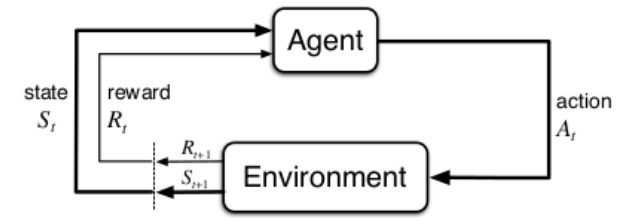
\includegraphics[width=0.6\textwidth]{img/rl_diagrama.png}
    \caption{Ciclo de interação entre agente e ambiente em Aprendizagem por Reforço \cite{sutton2018reinforcement}.}
    \label{fig:rl}
\end{figure}

Mapeamos o problema diagnóstico num MDP em tempo discreto com a biblioteca Gymnasium \cite{noauthor_gymnasium_nodate, towers_gymnasium_2023}. A epidemia avança em dias; dentro de cada dia, os casos que aguardam decisão são apresentados ao agente um por vez, de modo que cada passo do agente é uma decisão sobre um único caso. Como o estado verdadeiro da epidemia é ocultado pelo ruído clínico e pelo atraso dos laudos, o agente não observa $S_t$ diretamente, mas uma observação $O_t$ composta por: um tensor espacial de seis canais que resume os casos notificados, os exames realizados e os casos confirmados por laudo; as coordenadas do caso em avaliação; e um vetor de contexto com 16 posições --- o diagnóstico clínico do caso, os resultados dos exames já feitos, a confirmação epidemiológica, a densidade local de confirmados e uma estatística da evidência acumulada sobre o médico, descrita na Seção \ref{subsec:treino}. Opcionalmente, quatro variáveis temporais (fração do horizonte decorrida, casos notificados no dia, tendência dos últimos sete dias e idade do caso) podem ser acrescentadas; todas são lidas do que a vigilância observa, nunca da curva verdadeira do gerador.

\paragraph{Espaço de ações.} O agente escolhe, para cada caso, uma entre sete ações, agrupadas em três categorias (Figura \ref{fig:decision_flow}):
\begin{itemize}
    \item \textbf{Não agir:} a ação nula. Não consome recurso e deixa valer o diagnóstico do médico.
    \item \textbf{Investigar:} solicitar exame de dengue, exame de chikungunya ou confirmação epidemiológica. Toda investigação tem custo imediato, e o resultado só fica disponível depois.
    \item \textbf{Concluir:} afirmar que o caso é dengue, chikungunya ou ``outro'' (não arbovirose). A alegação vem da própria ação, e não do diagnóstico corrente, o que permite ao agente discordar do médico com base em outra evidência sem precisar de um exame para ``editar'' o rótulo.
\end{itemize}
A versão anterior tinha apenas ``confirmar'' e ``descartar'' o diagnóstico corrente. Com ela, trocar dengue por chikungunya exigia um exame mesmo quando os dados já indicavam a resposta: medimos que um classificador que infere pela posição e pelo palpite clínico ficava 11 pontos de acurácia abaixo do que atingiria se pudesse atribuir a classe diretamente --- pontos inacessíveis por falta de ação, e não de sinal.

\paragraph{Ciclo de vida do caso.} Um caso entra na fila do agente no dia em que é notificado. Se o agente solicita uma investigação, a amostra é colhida na hora, mas o laudo só amadurece cinco dias depois; \textbf{quando o laudo chega, o caso volta ao agente}, que decide de posse do resultado. O caso sai da fila quando o agente o conclui, quando o agente deixa de agir sobre ele ou quando o episódio termina; o número de retornos é limitado a dois, e, esgotada a investigação, as ações ficam restritas às conclusivas. O mecanismo de retorno é uma mudança substantiva em relação a uma formulação de visita única: se cada caso fosse apresentado uma só vez, pedir um exame significaria abrir mão da decisão sobre aquele caso --- o laudo seria aplicado automaticamente e o agente nunca mais o veria. Testar e decidir seriam mutuamente exclusivos, o que limita artificialmente a acurácia atingível (Seção \ref{subsec:ceiling}).

\begin{figure}[htbp]
    \centering
    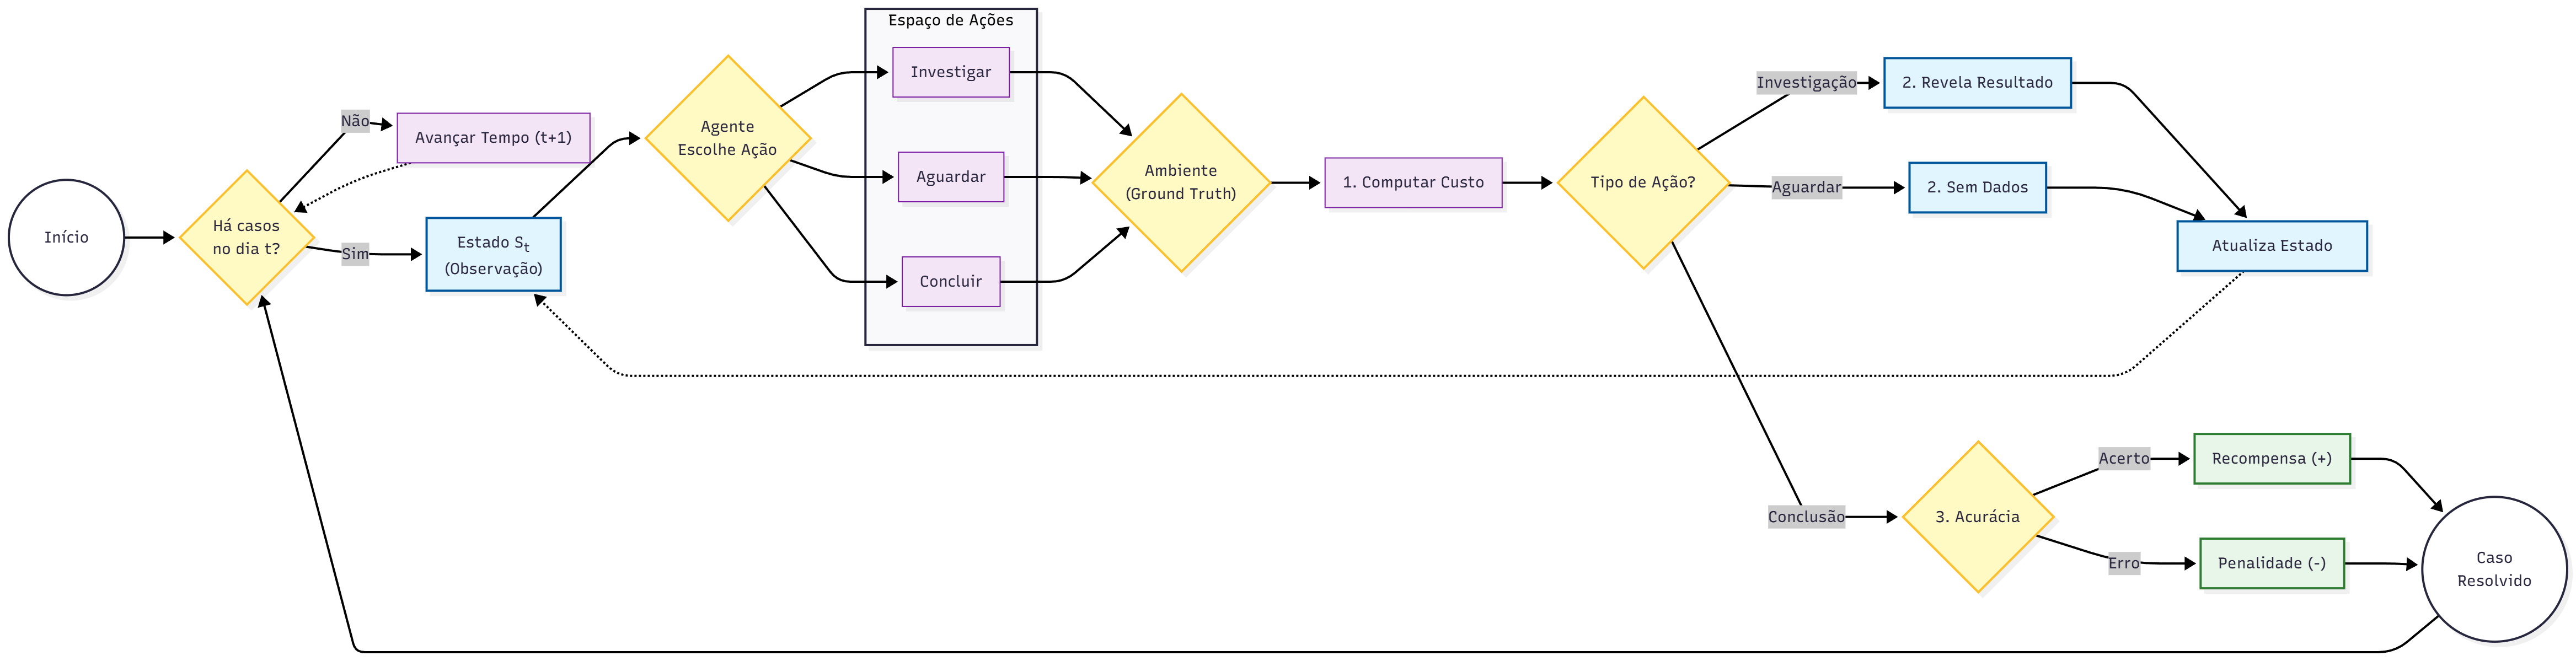
\includegraphics[width=0.95\textwidth]{img/agent_decision.png}
    \caption{Fluxo de decisão do agente.}
    \label{fig:decision_flow}
\end{figure}

\subsection{Função de recompensa}
\label{subsec:recompensa}

A recompensa traduz os dilemas logísticos e clínicos da vigilância epidemiológica em três camadas: um custo operacional imediato, o desfecho da decisão e um placar terminal.

\paragraph{Camada 1 --- Custo imediato.} Toda ação paga seu custo operacional no momento em que é tomada:
\begin{equation}
    C(a) = \begin{cases}
        c_{\text{exame}} = 4{,}0 & \text{exame de dengue ou de chikungunya}\\
        c_{\text{epi}} = 4{,}0 & \text{confirmação epidemiológica}\\
        0 & \text{não agir, concluir}
    \end{cases}
    \label{eq:costs}
\end{equation}
Não agir custa zero por decisão de projeto: é a ação nula no sentido usual de Aprendizagem por Reforço. Um custo pequeno e constante por inação, como havia em versões anteriores, somava uma deriva negativa sem informação sobre a ação mais frequente do agente.

\paragraph{Camada 2 --- Desfecho da decisão.} Apenas as ações conclusivas são pontuadas. Seja $y_c$ a doença verdadeira do caso, $\hat{y}$ a classe alegada e $\varnothing$ o rótulo ``não é arbovirose'':
\begin{equation}
    R_{\text{dec}}(c, \hat{y}) = \begin{cases}
        +10 & \hat{y} = y_c \quad \text{(decisão correta)}\\
        -30 & \hat{y} = \varnothing \land y_c \neq \varnothing \quad \text{(caso real descartado)}\\
        -20 & \text{demais erros}
    \end{cases}
    \label{eq:decision}
\end{equation}
Descartar um paciente que tinha arbovirose é um falso negativo de vigilância e recebe a penalidade mais pesada, refletindo o risco clínico assimétrico \cite{yu_deep_2023}. Concluir um caso que foi investigado rende ainda um bônus imediato de $+2$, que encurta a cadeia investigar--concluir.

Nas primeiras versões, esse desfecho era creditado cinco dias depois da decisão, para reproduzir o atraso entre decidir e conhecer a consequência. O atraso foi removido: como dezenas de desfechos amadureciam no mesmo dia, cada um caía num passo que pertencia a outro caso, e medimos que cerca de 90\% da variância da recompensa de um passo vinha de decisões tomadas dias antes, sobre outros pacientes. O atraso do \emph{laudo}, que é o que cria a investigação sequencial ``testar hoje, decidir quando o resultado voltar'', foi mantido.

\paragraph{Camada 3 --- Placar terminal.} Ao fim do episódio, cada caso contribui com $+1$ se o diagnóstico final estiver correto e $-3$ caso contrário:
\begin{equation}
    R_{\text{final}} = \sum_{c} \Big( \mathbb{I}[\hat{y}_c = y_c] - 3 \cdot \mathbb{I}[\hat{y}_c \neq y_c] \Big)
    \label{eq:terminal}
\end{equation}
Uma formulação anterior punia apenas os erros em casos que \emph{nunca haviam sido testados}. Isso transformava o exame em isenção: pedir um ensaio removia a penalidade mesmo quando o laudo voltava indeterminado e não mudava nada, premiando o ato de testar e não a informação obtida. Punir o erro em si elimina essa distorção.

\paragraph{Casos em aberto.} Um caso cuja investigação foi aberta --- com exame ou ida a campo --- e nunca concluída recebe $-10$, cobrado no passo em que o agente o abandona. Não agir sobre um caso não investigado, ao contrário, não é abandono: é deixar valer o diagnóstico do médico, uma decisão legítima, julgada pelo placar terminal. A distinção corrigiu um incentivo perverso: quando a penalidade recaía sobre todo caso não concluído e era somada em bloco no fim do episódio, de 62\% a 85\% dos casos terminavam em aberto, e a política ``clínica'', que apenas aceita o médico, pontuava $-4036{,}5$ no ambiente sintético; com a redefinição, passou a $-267{,}2$ e a superar a política de confirmar tudo. Abster-se tornou-se melhor que opinar mal, como deveria ser.

\paragraph{Custo do exame e escassez.} O parâmetro $c_{\text{exame}}$ governa se o problema de alocação existe. Com exame barato, testar todos é quase sempre ótimo e não há o que alocar; caro demais, o ambiente degenera e a melhor política passa a ser não agir. O valor $4{,}0$ foi escolhido por varredura empírica com políticas fixas no ambiente sintético: nele, investigar ainda compensa, mas com margem estreita --- o regime em que escolher \emph{quais} casos investigar rende mais. \todo{refazer a varredura do custo do exame no ambiente v9; a calibração atual foi feita no sintético}

\paragraph{Decomposição por caso.} O ambiente entrega, em cada passo, a recompensa atribuível à decisão daquele passo e publica, em paralelo, a que caso ela pertence, em que dia foi tomada e se o caso terminou. A parcela terminal de cada caso é atribuída a ele uma única vez. A soma das parcelas por caso reconstrói exatamente o total do episódio, inclusive a cauda dos casos que ficam abertos, de modo que a recompensa usada para comparar agentes é a mesma em todos os experimentos. Essa decomposição é a matéria-prima da atribuição de crédito descrita na Seção \ref{subsec:credito}.

\subsection{Agentes avaliados}

\paragraph{Políticas fixas.} O desempenho é comparado a um conjunto de políticas de referência que não aprendem. Elas são essenciais para interpretar os resultados: sem elas, um agente treinado pode parecer competente apenas por ser melhor que o acaso.
\begin{itemize}
    \item \textbf{Aleatória:} escolhe qualquer ação com igual probabilidade.
    \item \textbf{Clínica:} nunca age, aceitando o diagnóstico do médico sem exames. Mede o que a triagem clínica entrega sozinha e é o piso de referência.
    \item \textbf{Confirmar tudo} (\textit{confirmall}): conclui cada caso com o diagnóstico clínico, sem testar. Não melhora a acurácia, mas coleta o desfecho sempre que a triagem acerta.
    \item \textbf{Testar uma vez} (\textit{testonce}): solicita um exame por caso e conclui quando o laudo chega.
    \item \textbf{Testar duas vezes} (\textit{testtwice}): solicita os dois exames e conclui com os dois laudos em mãos.
\end{itemize}

\paragraph{Q-Learning tabular.} Atualiza o valor de cada par estado--ação pela equação de Bellman \cite{watkins1992q}:
$$ Q(S_t, A_t) \leftarrow Q(S_t, A_t) + \alpha \left[ R_{t+1} + \gamma \max_{a'} Q(S_{t+1}, a') - Q(S_t, A_t) \right]. $$
As dimensões da grade fazem o espaço de estados crescer de forma explosiva; a tabela resultante fica esparsa demais e o aprendizado se torna intratável pela maldição da dimensionalidade \cite{bellman1957dynamic}. Numa versão anterior do ambiente, o número de estados visitados ainda crescia ao fim do treino (3.237 estados), e a acurácia do agente ficou abaixo da do próprio diagnóstico clínico.

\paragraph{Deep Q-Network.} Para lidar com a alta dimensionalidade, substituímos a tabela por uma aproximação não linear com redes convolucionais \cite{mnih2015human, goodfellow2016deep}, minimizando o erro quadrático em relação a uma rede-alvo $\theta^-$:
$$ L_i(\theta_i) = \mathbb{E} \left[ \left( r + \gamma \max_{a'} Q(s', a'; \theta_{i}^-) - Q(s, a; \theta_i) \right)^2 \right]. $$
O DQN é mantido como controle: como mostramos na Seção \ref{subsec:dqn}, estabilizado, ele converge de forma confiável para uma política degenerada de inação.

\paragraph{Proximal Policy Optimization.} O PPO \cite{schulman2017ppo} otimiza diretamente uma política estocástica $\pi_\theta$, limitando o tamanho de cada atualização pela razão de probabilidades $\rho_t(\theta) = \pi_\theta(a_t \mid s_t)/\pi_{\theta_{\text{old}}}(a_t \mid s_t)$:
\begin{equation}
L^{\text{CLIP}}(\theta) = \mathbb{E}_t \Big[ \min\big( \rho_t(\theta) \hat A_t,\ \text{clip}(\rho_t(\theta), 1-\epsilon, 1+\epsilon)\, \hat A_t \big) \Big],
\end{equation}
em que $\hat A_t$ é uma estimativa da vantagem da ação tomada. Na forma usual, $\hat A_t$ é obtida pela estimativa de vantagem generalizada (GAE) \cite{schulman2016gae}, que encadeia passos \emph{consecutivos} da trajetória:
\begin{equation}
\delta_t = r_t + \gamma V(s_{t+1}) - V(s_t), \qquad \hat A_t = \sum_{k \ge 0} (\gamma\lambda)^k \delta_{t+k}.
\label{eq:gae}
\end{equation}
É exatamente essa escolha que a Seção \ref{subsec:credito} questiona.

\subsection{Atribuição de crédito por caso}
\label{subsec:credito}

\paragraph{O problema.} O agente decide um caso por passo, e os casos se sobrepõem no tempo. No ambiente de referência, há cerca de 30 decisões sobre \emph{outros} pacientes entre o exame de um caso e sua conclusão. Um exame devolve sempre apenas $-c_{\text{exame}}$; o benefício aparece dezenas de passos depois, num passo que pertence a outro paciente, e o GAE da Equação \eqref{eq:gae} obriga esse valor a atravessar as decisões alheias, somando o ruído de cada uma. Medimos diretamente o efeito: no passo de cada exame, a correlação entre o retorno e o fato de o exame ter levado ao diagnóstico correto é de $-0{,}019$ quando o retorno é o global, descontado por passo, e de $0{,}994$ quando é o retorno do próprio caso, descontado por dia. O sinal existe na trajetória; a definição usual de retorno o apaga.

Essa leitura explica por que três tentativas anteriores falharam pela mesma razão. A modelagem de recompensa por potencial \cite{ng1999policy} não se aplica: como o estado seguinte já é outro paciente, o potencial se cancela no mesmo passo, e com cerca de 250 investigações abertas a deriva $(1-\gamma)\Phi$ supera o incremento pretendido para qualquer escala escolhida. O crédito retroativo exigiria reescrever recompensa já entregue, o que não é implementável num MDP \textit{online}. E baratear o exame, dobrando a margem de investigar, não fez o agente pedir um exame sequer. A saída mais simples --- um episódio por caso --- resolveria a intercalação destruindo justamente a dinâmica temporal da epidemia, que é o objeto deste trabalho; ela foi descartada. A intercalação foi resolvida no aprendiz, e não no ambiente.

\paragraph{O método.} Cada transição traz a identificação do episódio e do caso, o dia $d$ da decisão e a parcela $r^{\text{caso}}$ da recompensa que pertence àquele caso. O \texttt{PerCasePPO} agrupa as transições do lote por (episódio, caso) e calcula o GAE ao longo da linha do tempo de \emph{cada paciente}, com o desconto elevado aos dias decorridos entre as decisões, e não aos passos. Para as posições $j$ de um mesmo caso:
\begin{align}
\text{desconto}_j &= \gamma^{\,d_{j+1} - d_j}, \nonumber\\
\delta_j &= r^{\text{caso}}_j + \text{desconto}_j \cdot V(s_{j+1}) - V(s_j), \label{eq:gae_caso}\\
\hat A_j &= \delta_j + \text{desconto}_j \cdot \lambda \cdot \hat A_{j+1}. \nonumber
\end{align}
No último passo de um caso dentro do lote, se o caso terminou não há futuro; se o lote cortou sua linha do tempo, faz-se \textit{bootstrap} com o próprio valor e um dia de desconto. A estrutura é a mesma da atribuição de crédito em sistemas multiagente: cada caso é tratado como um agente que compartilha o mundo com os demais.

Duas invariâncias sustentam o método e são verificadas por testes automatizados. A primeira é que \textbf{a recompensa do ambiente não muda}: a soma das parcelas por caso reconstrói o total do episódio, e a métrica de comparação continua canônica. A segunda é que \textbf{a vantagem de um caso não depende da intercalação}: inserir 30 decisões ruidosas sobre outros pacientes entre dois passos do caso $X$ não altera a vantagem de $X$.

\paragraph{Limitação.} O crédito por caso ignora a externalidade do exame: cada laudo positivo alimenta o mapa de confirmados e melhora a confirmação epidemiológica de casos \emph{futuros} na região, e esse ganho não volta para o caso que pagou o exame. Nas medições atuais o efeito é pequeno, pois o agente praticamente não usa a confirmação epidemiológica, mas é uma limitação real do método. \todo{quantificar a externalidade do exame não capturada pelo crédito por caso}

\subsection{Arquitetura e treinamento}
\label{subsec:treino}

Todos os agentes profundos usam o mesmo tronco de rede, a \textit{DengueNet}: camadas convolucionais processam o tensor espacial para extrair densidades e agrupamentos geográficos, e um ramo denso processa as coordenadas e o vetor de contexto do caso, em linha com arquiteturas que combinam mapas de risco e características individuais \cite{frommeyer_reinforcement_2025}. A pilha convolucional termina num \textit{pooling} adaptativo que fixa a saída em $64 \times 6 \times 6$ independentemente da resolução do mapa. Como a resolução extra é descartada pela própria arquitetura, o mapa é entregue à rede em $100 \times 100$ (o mundo continua $400 \times 400$): isso reduziu cada observação de 937,5 para 58,6 KB e o tempo de uma época de treino de 6min20 para 1min14, com apenas 1,7\% dos casos colidindo na mesma célula no mapa real.

\paragraph{Variáveis de contexto.} A competência do médico é latente, mas determina se vale testar. Expomos ao agente um resumo de duas posições da evidência acumulada no episódio: a taxa de concordância entre os laudos e o palpite clínico e a força dessa evidência (número de laudos informativos, com saturação). Essa estatística acompanha a competência verdadeira do médico com correlação de $+0{,}99$. A informação já estava implícita na observação, mas espalhada por um mapa esparso e, portanto, impraticável de extrair por convolução. Para estimar a competência, o agente precisa gastar alguns exames cedo, o que introduz um equilíbrio natural entre exploração e aproveitamento.

\paragraph{Treinamento do PPO.} Usamos a biblioteca Tianshou \cite{weng2021tianshou}, com 300 mil passos por treino (10 épocas de 30 mil), taxa de aprendizado $3 \times 10^{-4}$, $\gamma = 0{,}99$, $\lambda = 0{,}95$, $\epsilon = 0{,}2$, coeficiente de entropia 0,02, lotes de 256 transições e 8 ambientes de treino em paralelo. A máscara de ações, que força a conclusão ao fim da investigação, é aplicada diretamente nos \textit{logits} do ator --- sem isso, o PPO ignoraria a máscara e resolveria silenciosamente um problema mais fácil. Como dezenas de desfechos de centenas de casos compõem retornos da ordem de milhares, a recompensa é multiplicada por uma constante (0,10) \emph{apenas no treino}, e a mesma escala é aplicada às parcelas por caso usadas no GAE; multiplicar por uma constante positiva não altera a política ótima, e toda avaliação usa a escala original.

\paragraph{Braços do experimento.} Para separar o efeito do crédito do efeito da informação temporal, treinamos três braços no mesmo ambiente, com a mesma rede e os mesmos hiperparâmetros (Tabela \ref{tab:bracos}). O par A $\times$ C isola a atribuição de crédito, com observação idêntica; o par B $\times$ C isola as variáveis temporais, com crédito idêntico. No ambiente corrigido (v9), os braços A e C foram retreinados com o mesmo procedimento, mas com uma única semente de treino cada; o braço B não foi repetido, pois as variáveis temporais não contribuíram no v8.

\begin{table}[htbp]
\centering
\begin{tabular}{llll}
\toprule
\textbf{Braço} & \textbf{Crédito} & \textbf{Contexto observado} & \textbf{Seeds} \\ \midrule
A & GAE usual (Eq.~\ref{eq:gae}) & 16 posições & 4 \\
B & por caso, em dias (Eq.~\ref{eq:gae_caso}) & 16 + 4 temporais & 3 \\
C & por caso, em dias (Eq.~\ref{eq:gae_caso}) & 16 posições (= A) & 4 \\ \bottomrule
\end{tabular}
\caption{Braços de treino do PPO no ambiente v8. No v9, A e C têm uma semente de treino cada.}
\label{tab:bracos}
\end{table}

\subsection{Protocolo de avaliação}
\label{subsec:protocolo}

\paragraph{Cenários pareados.} Os agentes são avaliados em 10 cenários epidêmicos de teste, cada um identificado por uma semente fixa (100, 150, \ldots, 550). Como a semente reproduz o mesmo surto, o mesmo médico e o mesmo ruído clínico para todos os agentes, as comparações são \textbf{pareadas}, o que é consideravelmente mais poderoso do que comparar médias independentes --- precaução necessária diante da variância discutida na Seção \ref{subsec:confounder}. Um segundo conjunto, de 12 cenários com sementes nunca usadas antes (9001 em diante), testa a generalização.

\paragraph{Checkpoint.} Avalia-se sempre o checkpoint \emph{final} do treino, nunca o de melhor desempenho durante o treino: medimos que este último fica 1.000 a 1.460 pontos acima do final no DQN --- ele seleciona ruído.

\paragraph{Bootstrap hierárquico e pareado.} Há duas fontes de variância: a semente que treinou o agente e o surto em que ele é avaliado. Os intervalos de confiança são obtidos por bootstrap hierárquico \cite{saravanan2020hierarchical}, que reamostra primeiro as sementes de treino e depois os episódios de avaliação. A reamostragem dos episódios é \emph{compartilhada} entre braços em cada réplica, preservando o pareamento, enquanto as sementes de treino, que são treinos independentes, são reamostradas separadamente por braço. Seguindo \citeonline{agarwal2021precipice}, reportamos a média e a média interquartil (IQM), robusta a episódios catastróficos; a diferença de médias entre braços; e a probabilidade de melhoria $P(X > Y)$, a chance de um episódio de $X$ superar o mesmo episódio de $Y$, sobre todos os pares de sementes de treino, com empate valendo 1/2. Usamos intervalos percentis de 95\% com 10 mil réplicas.

Uma limitação precisa ser declarada: com três ou quatro sementes de treino, o nível superior do bootstrap tem pouca resolução (três sementes admitem apenas dez reamostras distintas), e o intervalo tende a ser estreito demais nesse nível. Os intervalos reportados são honestos quanto ao surto e otimistas quanto à semente de treino. No v9, com uma semente por braço, o bootstrap reamostra apenas os episódios, e o intervalo não captura a variação entre sementes de treino; no v8, essa variação foi pequena diante das diferenças reportadas no v9 (desvio entre sementes de cerca de 50 pontos no braço C e de 130 no A). \todo{treinar ao menos 4--5 seeds por braço, no v9, para dar resolução ao nível superior do bootstrap}

\paragraph{Métricas.} A métrica primária é a recompensa acumulada por episódio, que agrega os compromissos logísticos e clínicos da política. As secundárias são a acurácia multiclasse e o número de exames solicitados por episódio. Uma ressalva se aplica à acurácia: embora calculada sobre três classes (dengue, chikungunya, outro), no ambiente v8 a verdade só contém dengue e chikungunya (Seção \ref{subsec:ressalva}); nele a métrica é, na prática, binária, e qualquer atribuição de ``outro'' conta como erro. No v9 ela passa a medir de fato as três classes.

\subsection{Implementação computacional e reprodutibilidade}

Os experimentos foram desenvolvidos em Python 3.12, com NumPy e Pandas para o processamento de dados, PyTorch para as redes e Tianshou para os algoritmos de Aprendizagem por Reforço. O treinamento foi executado numa máquina com GPU NVIDIA RTX 3060 (12\,GB) e 32\,GB de RAM; cada semente de treino do PPO leva cerca de três horas, com o laço limitado pelo ambiente, e não pela rede. Todas as fontes de aleatoriedade (gerador, Gymnasium e inicialização das redes) são controladas por semente, e todo parâmetro do ambiente relatado aqui é definido em arquivos de configuração, não no código. O comportamento do ambiente é travado por uma suíte de 259 testes automatizados. O código-fonte completo será disponibilizado em repositório público institucional.

% =====================================================================
\section{Resultados e Discussão}
% =====================================================================

\noindent\textbf{Nota sobre o estado dos resultados.} As Seções \ref{subsec:ceiling} a \ref{subsec:temperatura} reportam resultados do ambiente v8 (SEIR e \textit{kriging}), que, como descrito na Seção \ref{subsec:ressalva}, não continha casos não arbovirais. A Seção \ref{subsec:v9} reporta o ambiente corrigido (v9), com uma semente de treino por braço. Ambos devem ser lidos como preliminares; a reavaliação completa no v9 (mais sementes, anos e temperatura) está em andamento (Seção \ref{sec:todo}).

\subsection{O teto de informação do ambiente}
\label{subsec:ceiling}

Antes de comparar agentes, é preciso estabelecer o que é alcançável. Como cada exame tem sensibilidade $s$ e uma fração $p$ de laudos indeterminados (que preservam o palpite clínico), a acurácia máxima obtida testando todos os casos é aproximadamente
$$ \text{acc}_{\max} \approx (1 - p)\, s + p \cdot \text{acc}_{\text{clínica}}. $$
Com os parâmetros de RT-PCR isso corresponde a $\approx 0{,}96$, confirmado empiricamente pela política \textit{testonce} (0,960). É um limite de \textbf{informação do ambiente}, e não do algoritmo. Vale registrar que, sob uma configuração anterior --- exame com sensibilidade e especificidade de 0,90, 10\% de laudos indeterminados e sem retorno do caso --- esse teto era de apenas 0,873, o que tornava inatingível a meta de 90\% de acurácia. O ganho veio da modelagem do exame e do ciclo de vida do caso, não do algoritmo de aprendizado. Note-se que esse teto supõe que um exame basta para resolver o caso, o que só vale na ausência de casos não arbovirais (ambiente v8). No ambiente corrigido (v9), \textit{testonce} cai para 0,756 de acurácia, e são precisos os dois exames para chegar a 0,938 (\textit{testtwice}; Seção \ref{subsec:v9}). \todo{derivar analiticamente o teto de informação do v9, com três classes e dois exames}

\subsection{A competência do médico domina a variância}
\label{subsec:confounder}

Numa fase anterior do projeto, ao comparar o ambiente sintético com o \textit{kriging}, observou-se desempenho superior no segundo --- resultado contraintuitivo, já que se esperava maior dificuldade na distribuição real. A investigação mostrou tratar-se de um artefato: com a mesma semente, a competência clínica sorteada é idêntica nos dois ambientes, e ainda assim o \emph{baseline} clínico, que sequer usa informação espacial, variava entre 0,690 e 0,731 de acurácia. A explicação está na correlação entre a competência sorteada do médico e a recompensa do episódio: $+0{,}974$ para o DQN e $+0{,}977$ para o \emph{baseline} clínico. Cerca de 97\% da variação observada decorria do médico sorteado, e não da política avaliada. Esse achado justifica duas decisões metodológicas mantidas em todos os experimentos: comparações pareadas por semente e um bootstrap que reamostra os episódios de forma compartilhada entre braços (Seção \ref{subsec:protocolo}).

\subsection{Do DQN ao PPO: o algoritmo como primeiro gargalo}
\label{subsec:dqn}

O DQN apresentou instabilidade real, com a recompensa oscilando até 6.300 pontos entre avaliações vizinhas. A troca da perda quadrática pela de Huber a estabilizou de forma inequívoca (de $\pm 1340$ para $\pm 9$ entre sementes), e o resultado \emph{piorou}: estabilizado, o DQN convergiu de forma confiável para um ótimo local degenerado, com 66,7\% de inação e nenhum exame. Com o mesmo ambiente, o mesmo tronco de rede e a mesma máscara de ações, o PPO com GAE usual foi o primeiro agente treinado a superar a política de não agir (Tabela \ref{tab:dqn_ppo}), com curva de treino monotônica. Ajustes de taxa de aprendizado, tamanho do \textit{buffer}, retornos de $n$ passos e frequência de atualização da rede-alvo não moveram o DQN de forma mensurável; o ganho veio de mudar de algoritmo, não de girar botões.

\begin{table}[htbp]
\centering
\begin{tabular}{lrrl}
\toprule
\textbf{Agente} & \textbf{Recompensa} & \textbf{Acurácia} & \textbf{Comportamento} \\ \midrule
DQN (Huber, controle) & $-4164 \pm 9$ & 0,55 & converge para a inação \\
PPO (GAE usual) & $+632 \pm 43$ & 0,73 & curva monotônica \\ \bottomrule
\end{tabular}
\caption{DQN e PPO no mesmo ambiente sintético (versão anterior ao SEIR), média $\pm$ desvio entre sementes de treino. O resultado do PPO se reproduziu com sementes novas e mais treino ($+645{,}6 \pm 76{,}0$, três sementes, 300 mil passos).}
\label{tab:dqn_ppo}
\end{table}

O PPO, porém, quase não pedia exames. No sintético, chegou a $+632$ sem pedir exame algum, aprendendo a discordar do médico pela posição do caso --- a geografia, com 93,7\% de acerto, entregava a resposta de graça. Na distribuição real do Rio, com o mesmo algoritmo, o agente pedia de 7 a 37 exames por episódio, contra cerca de 370 da política \textit{testonce}. Corrigir o modelo epidêmico (Seção \ref{subsec:seir}) tampouco resolveu: o braço A, treinado no ambiente com SEIR, manteve o padrão de subinvestimento. O gargalo restante era a atribuição de crédito.

\subsection{Atribuição de crédito: resultado principal}
\label{subsec:resultado_credito}

A Tabela \ref{tab:resultado_v8} resume o desempenho no ambiente de referência, e a Tabela \ref{tab:comparacoes_v8} as comparações pareadas que o experimento foi desenhado para responder.

\begin{table}[htbp]
\centering
\resizebox{\textwidth}{!}{%
\begin{tabular}{lcrrr}
\toprule
\textbf{Agente} & \textbf{Seeds} & \textbf{Recompensa [IC 95\%]} & \textbf{Acurácia [IC 95\%]} & \textbf{Exames [IC 95\%]} \\ \midrule
\textit{Testonce} (melhor política fixa) & -- & $+2782$ [$+2668$; $+2900$] & 0,960 [0,953; 0,966] & 369 [353; 384] \\
\textbf{C --- crédito por caso} & 4 & $\mathbf{+2692}$ [$+2523$; $+2842$] & 0,937 [0,923; 0,950] & 284 [223; 335] \\
B --- crédito por caso + tempo & 3 & $+2649$ [$+2413$; $+2842$] & 0,931 [0,908; 0,946] & 266 [206; 321] \\
\textit{Testtwice} & -- & $+1051$ [$+969$; $+1135$] & 0,950 [0,945; 0,954] & 737 [706; 768] \\
A --- GAE usual & 4 & $+684$ [$-146$; $+1498$] & 0,739 [0,674; 0,803] & 25 [5; 64] \\
\textit{Confirmall} & -- & $+346$ [$-656$; $+1335$] & 0,710 [0,633; 0,789] & 0 \\
Clínica (piso de referência) & -- & $-64$ [$-184$; $+54$] & 0,710 [0,633; 0,789] & 0 \\ \bottomrule
\end{tabular}%
}
\caption{Desempenho no ambiente de referência v8 (\textit{kriging} e SEIR), 10 cenários pareados. Médias com intervalos de confiança de 95\% por bootstrap hierárquico e pareado (10 mil réplicas); checkpoint final de cada semente de treino. Resultados preliminares: o v8 não contém casos não arbovirais (Seção \ref{subsec:ressalva}).}
\label{tab:resultado_v8}
\end{table}

\begin{table}[htbp]
\centering
\resizebox{\textwidth}{!}{%
\begin{tabular}{lrcrr}
\toprule
\textbf{$X$ contra $Y$} & \textbf{$\Delta$ Recompensa [IC 95\%]} & \textbf{$P(X>Y)$} & \textbf{$\Delta$ Exames [IC 95\%]} & \textbf{$\Delta$ Acurácia [IC 95\%]} \\ \midrule
C $\times$ A (efeito do crédito) & $+2009$ [$+1197$; $+2882$] & 1,00 & $+259$ [$+205$; $+305$] & $+0{,}199$ [$+0{,}130$; $+0{,}269$] \\
B $\times$ C (efeito das variáveis temporais) & $-43$ [$-196$; $+85$] & 0,47 & $-19$ [$-53$; $+12$] & $-0{,}007$ [$-0{,}024$; $+0{,}007$] \\
C $\times$ \textit{testonce} & $-90$ [$-250$; $+67$] & 0,38 & $-84$ [$-141$; $-38$] & $-0{,}022$ [$-0{,}039$; $-0{,}007$] \\
A $\times$ clínica & $+748$ [$+27$; $+1446$] & 0,68 & $+25$ [$+5$; $+64$] & $+0{,}028$ [$+0{,}005$; $+0{,}072$] \\ \bottomrule
\end{tabular}%
}
\caption{Comparações pareadas episódio a episódio no ambiente v8. $P(X>Y)$ é a probabilidade de um episódio de $X$ superar o mesmo episódio de $Y$ (empate vale 1/2).}
\label{tab:comparacoes_v8}
\end{table}

Os contrastes licenciam três conclusões. \textbf{Primeira: o ganho vem da atribuição de crédito.} Entre A e C a única diferença é o crédito, e C supera A em $+2009$ pontos, com $P(C > A) = 1{,}00$; o agente passa de 25 para 284 exames por episódio e ganha cerca de 20 pontos de acurácia. É o primeiro agente do projeto que investiga. \textbf{Segunda: as variáveis temporais não contribuíram.} B e C são indistinguíveis ($-43$ [$-196$; $+85$], $P = 0{,}47$). Isso não prova que informação temporal seja inútil, apenas que estas quatro variáveis, com este crédito, não acrescentaram. \textbf{Terceira: o agente C empata com a melhor política fixa usando menos exames.} A diferença de recompensa para \textit{testonce} não é distinguível de zero ($-90$ [$-250$; $+67$]), com 84 exames a menos por episódio e 2,2 pontos percentuais a menos de acurácia --- o agente não testa todos os casos, escolhe quais investigar.

A estabilidade também separa os braços (Figura \ref{fig:bracos}). O desvio entre sementes de treino é de cerca de 49 pontos nos braços com crédito por caso. O braço A, além de pior em média, colapsa em episódios específicos --- nos cenários 150, 250 e 550 chega a $-2200$ ---, enquanto o C nunca colapsa. A Figura \ref{fig:ultimo_dia} mostra o mecanismo num desses cenários: com um médico de especificidade 0,50, o agente A, que praticamente não investiga, herda os erros da triagem, enquanto o C investiga a maior parte dos casos; com um médico de especificidade 0,90, o C investiga apenas um quarto dos casos e ainda assim supera o \textit{testonce} naquele episódio.

\begin{figure}[htbp]
\centering
\includegraphics[width=\textwidth]{../results/demo/bracos.png}
\caption{Recompensa (à esquerda; pontos são sementes de treino) e exames por episódio (à direita) dos três braços do PPO no ambiente v8. As linhas indicam \textit{testonce} e a política clínica.}
\label{fig:bracos}
\end{figure}

\begin{figure}[htbp]
\centering
\includegraphics[width=\textwidth]{../results/demo/ultimo_dia.png}
\caption{Último dia da epidemia em dois cenários do ambiente v8, com a decisão final sobre cada caso: círculos são casos investigados e cruzes, não investigados; verde indica acerto e vermelho, erro. O número sob cada painel é a recompensa do episódio. Na linha superior (médico de especificidade 0,50), o agente A, que quase não investiga, herda os erros da triagem.}
\label{fig:ultimo_dia}
\end{figure}

Uma ablação sem retreino indica de onde vem a decisão: zerar o mapa espacial inteiro muda apenas de 0 a 2\% das decisões do agente. A política decide pelo vetor de contexto do caso; o mapa, nas condições atuais, é decorativo. \todo{incorporar os demais testes de robustez já executados (qualidade do médico, custo do exame, atraso do laudo, orçamento, ablação de entradas) depois de refeitos no v9}

\paragraph{Generalização para cenários inéditos.} Em 12 cenários com sementes nunca usadas, o padrão se mantém: C $\times$ A $= +1653$ [$+1072$; $+2313$], $P = 1{,}00$, e C $\times$ \textit{testonce} $= +6$ [$-124$; $+149$], novamente um empate estatístico ($+2616$ contra $+2611$ de média), com 81 exames a menos.

\subsection{Consistência entre anos}
\label{subsec:anos}

Sem retreino, avaliamos os agentes em superfícies de \textit{kriging} estimadas com notificações de outros anos (Tabela \ref{tab:anos}). Os resultados são praticamente idênticos aos da referência. O motivo é que as três superfícies são igualmente pouco informativas: a posição, sozinha, acerta a doença em 53--54\% em todas elas, e as superfícies de dengue de 2015 e 2016 têm correlação de 0,90. A consistência é, portanto, uma verificação de que a política não depende da geografia específica de um ano, e não um teste de generalização para cenários de dificuldade diferente --- esse é o papel da varredura da Seção \ref{subsec:temperatura}.

\begin{table}[htbp]
\centering
\resizebox{\textwidth}{!}{%
\begin{tabular}{lrrrcr}
\toprule
\textbf{Superfície} & \textbf{C} & \textbf{A} & \textbf{C $\times$ A [IC 95\%]} & \textbf{$P(C>A)$} & \textbf{C $\times$ \textit{testonce} [IC 95\%]} \\ \midrule
Referência (dengue e chik 2015--2016) & $+2692$ & $+684$ & $+2009$ [$+1197$; $+2882$] & 1,00 & $-90$ [$-250$; $+67$] \\
Dengue 2015 + chik 2016 & $+2710$ & $+634$ & $+2077$ [$+1161$; $+3081$] & 0,98 & $-72$ [$-236$; $+73$] \\
Rio 2016 & $+2721$ & $+699$ & $+2022$ [$+1163$; $+2950$] & 1,00 & $-61$ [$-226$; $+96$] \\ \bottomrule
\end{tabular}%
}
\caption{Avaliação sem retreino em superfícies de \textit{kriging} de anos diferentes (ambiente v8, 10 cenários pareados). A chikungunya entra só com 2016, pois circulou muito pouco no Rio em 2015.}
\label{tab:anos}
\end{table}

\subsection{Varredura de dificuldade espacial}
\label{subsec:temperatura}

Para medir o efeito da informatividade da geografia, variamos a temperatura $\tau$ das superfícies (Seção \ref{subsec:espacial}), de $\tau=0$ (posição não informa nada, acurácia de Bayes 0,50) a $\tau=32$ (0,94, o nível de separação do sintético, obtido às custas de concentrar cada doença em poucas células --- um extremo artificial); o treino ocorreu em $\tau=1$ (0,544). Sem retreino, a vantagem do crédito por caso é robusta em toda a faixa: C $\times$ A fica entre $+2000$ e $+2350$, com $P(C>A)$ entre 0,89 e 1,00 (Tabela \ref{tab:temperatura}). Por outro lado, a recompensa do C permanece essencialmente plana, em torno de $+2700$: o agente não explora a geografia mais informativa, o que é esperado, já que foi treinado num mundo em que a posição quase não informava. Em $\tau=8$, duas sementes do C degradam, o que alarga o intervalo --- instabilidade fora da distribuição de treino. A pergunta que esta varredura ainda não responde é se o crédito por caso vence o GAE usual quando cada um é \emph{treinado} em cada cenário, e se o agente aprende a usar uma geografia informativa quando ela existe.

\begin{table}[htbp]
\centering
\resizebox{\textwidth}{!}{%
\begin{tabular}{rcrrrcr}
\toprule
$\boldsymbol{\tau}$ & \textbf{Acerto da posição} & \textbf{C} & \textbf{A} & \textbf{C $\times$ A [IC 95\%]} & \textbf{$P(C>A)$} & \textbf{C $\times$ \textit{testonce} [IC 95\%]} \\ \midrule
0   & 0,500 & $+2718$ & $+670$ & $+2047$ [$+1198$; $+2953$] & 0,97 & $-65$ [$-242$; $+114$] \\
0,5 & 0,522 & $+2726$ & $+716$ & $+2010$ [$+1154$; $+2936$] & 0,95 & $-57$ [$-242$; $+128$] \\
1 (treino) & 0,544 & $+2692$ & $+691$ & $+2001$ [$+1194$; $+2885$] & 1,00 & $-90$ [$-250$; $+68$] \\
2   & 0,586 & $+2739$ & $+657$ & $+2083$ [$+1220$; $+3039$] & 1,00 & $-43$ [$-258$; $+134$] \\
4   & 0,651 & $+2651$ & $+503$ & $+2149$ [$+1258$; $+3094$] & 0,95 & $-131$ [$-468$; $+115$] \\
8   & 0,740 & $+2396$ & $+277$ & $+2119$ [$+969$; $+3380$] & 0,89 & $-387$ [$-1123$; $+162$] \\
16  & 0,852 & $+2686$ & $+334$ & $+2353$ [$+1301$; $+3579$] & 0,96 & $-96$ [$-484$; $+159$] \\
32  & 0,939 & $+2686$ & $+541$ & $+2145$ [$+1223$; $+3148$] & 0,95 & $-96$ [$-740$; $+227$] \\ \bottomrule
\end{tabular}%
}
\caption{Varredura da temperatura $\tau$ das superfícies de \textit{kriging}, sem retreino (ambiente v8, 10 cenários pareados). ``Acerto da posição'' é a acurácia de Bayes de um classificador que vê só a posição. A linha $\tau=1$ é uma reavaliação independente e difere ligeiramente da Tabela \ref{tab:resultado_v8}.}
\label{tab:temperatura}
\end{table}

\begin{figure}[htbp]
\centering
\figpendente{figura da curva de temperatura: recompensa de C, A e \textit{testonce} contra o acerto da posição, com ICs}
\caption{Recompensa em função da informatividade espacial.}
\label{fig:temperatura}
\end{figure}

\subsection{Uma ressalva crítica: o ambiente v8 não tinha casos não arbovirais}
\label{subsec:ressalva}

A configuração do ambiente de referência declarava uma prevalência de 25\% de casos não arbovirais, mas o gerador por \textit{kriging} ignorava esse parâmetro: todos os episódios do v8 continham apenas dengue e chikungunya, enquanto o gerador sintético produzia cerca de 123 casos ``outro'' por episódio. Sem eles, um laudo negativo de dengue implica logicamente chikungunya; um exame sempre basta, e concluir ``não é arbovirose'' nunca é correto.

Essa ausência reinterpreta três observações. A primeira é a inversão dos \emph{baselines} entre os ambientes (Tabela \ref{tab:baselines}): \textit{testonce} é ótimo no \textit{kriging} v8, e \textit{testtwice} no sintético. Atribuímos inicialmente essa inversão à geografia; ela decorre da presença ou ausência dos casos ``outro'' --- é com eles que o segundo exame passa a ser informativo. O ambiente corrigido confirma essa leitura: com os casos ``outro'', o \textit{kriging} v9 volta à mesma ordem do sintético, com \textit{testtwice} à frente e \textit{testonce} caindo de $+2782$ para $+322$, sem que a geografia tenha mudado. A segunda é a falha do agente C transferido sem retreino para o ambiente sintético ($-340$): ele aprendeu num mundo em que um exame resolve o caso. A terceira é a própria proximidade entre C e \textit{testonce}, cuja otimalidade no v8 decorre dessa simplificação.

\begin{table}[htbp]
\centering
\begin{tabular}{lrrr}
\toprule
\textbf{Política fixa} & \textbf{\textit{Kriging} v8} & \textbf{\textit{Kriging} v9} & \textbf{Sintético} \\
 & \textbf{(sem ``outro'')} & \textbf{(com ``outro'')} & \textbf{(com ``outro'')} \\ \midrule
\textit{Testonce} & $\mathbf{+2782}$ & $+322$ & $+473$ \\
\textit{Testtwice} & $+1051$ & $\mathbf{+1225}$ & $\mathbf{+1249}$ \\
\textit{Confirmall} & $+346$ & $-1734$ & $-1821$ \\
Clínica & $-64$ & $-344$ & $-355$ \\ \bottomrule
\end{tabular}
\caption{Políticas fixas nos geradores com SEIR (10 cenários pareados). A ordem entre \textit{testonce} e \textit{testtwice} se inverte no \textit{kriging} v8, o único sem casos não arbovirais, e volta à ordem do sintético no v9.}
\label{tab:baselines}
\end{table}

A comparação entre os braços A e C não é afetada por essa ressalva no que tem de essencial: ambos foram treinados e avaliados no mesmo ambiente, com observação idêntica, e o contraste isola a atribuição de crédito. Mas o problema de alocação que o v8 colocava era mais simples do que o pretendido --- descobrir que investigar compensa, e não até onde aprofundar a investigação ---, e os números das seções anteriores devem ser lidos nesse contexto. A Seção \ref{subsec:v9} mostra o que acontece quando a investigação passa a ter profundidade.

\subsection{Resultados no ambiente corrigido (v9)}
\label{subsec:v9}

O ambiente v9 é idêntico ao v8, exceto pelos casos não arbovirais, que passam a representar cerca de um quarto das notificações (Seção \ref{subsec:espacial}). Os braços A e C foram retreinados com o procedimento do v8 (PPO, 300 mil passos, checkpoint final), com uma única semente de treino cada, e avaliados nos mesmos 10 cenários pareados (Tabelas \ref{tab:resultado_v9} e \ref{tab:comparacoes_v9}).

\begin{table}[htbp]
\centering
\resizebox{\textwidth}{!}{%
\begin{tabular}{lcrrr}
\toprule
\textbf{Agente} & \textbf{Seeds} & \textbf{Recompensa [IC 95\%]} & \textbf{Acurácia [IC 95\%]} & \textbf{Exames [IC 95\%]} \\ \midrule
\textbf{C --- crédito por caso} & 1 & $\mathbf{+2387}$ [$+2186$; $+2564$] & 0,938 [0,929; 0,947] & 675 [633; 716] \\
\textit{Testtwice} (melhor política fixa) & -- & $+1225$ [$+1131$; $+1315$] & 0,938 [0,933; 0,943] & 978 [938; 1014] \\
\textit{Testonce} & -- & $+322$ [$+219$; $+431$] & 0,756 [0,750; 0,763] & 489 [469; 507] \\
Clínica (piso de referência) & -- & $-344$ [$-459$; $-225$] & 0,576 [0,521; 0,635] & 0 \\
\textit{Confirmall} & -- & $-1734$ [$-2694$; $-730$] & 0,576 [0,521; 0,635] & 0 \\
A --- GAE usual & 1 & $-1972$ [$-2897$; $-1028$] & 0,563 [0,511; 0,619] & 6 [2; 11] \\ \bottomrule
\end{tabular}%
}
\caption{Desempenho no ambiente v9 (\textit{kriging} e SEIR, com casos não arbovirais), 10 cenários pareados. Intervalos de 95\% por bootstrap pareado sobre os episódios (10 mil réplicas). Com uma semente de treino por braço, os intervalos não capturam a variação entre sementes de treino.}
\label{tab:resultado_v9}
\end{table}

\begin{table}[htbp]
\centering
\resizebox{\textwidth}{!}{%
\begin{tabular}{lrcrr}
\toprule
\textbf{$X$ contra $Y$} & \textbf{$\Delta$ Recompensa [IC 95\%]} & \textbf{$P(X>Y)$} & \textbf{$\Delta$ Exames [IC 95\%]} & \textbf{$\Delta$ Acurácia [IC 95\%]} \\ \midrule
C $\times$ \textit{testtwice} & $+1163$ [$+980$; $+1330$] & 1,00 & $-303$ [$-326$; $-281$] & $-0{,}000$ [$-0{,}009$; $+0{,}008$] \\
C $\times$ \textit{testonce} & $+2065$ [$+1796$; $+2299$] & 1,00 & $+186$ [$+158$; $+212$] & $+0{,}182$ [$+0{,}169$; $+0{,}194$] \\
C $\times$ A (efeito do crédito) & $+4359$ [$+3434$; $+5276$] & 1,00 & $+669$ [$+628$; $+710$] & $+0{,}374$ [$+0{,}319$; $+0{,}428$] \\
A $\times$ clínica & $-1627$ [$-2436$; $-800$] & 0,10 & $+6$ [$+2$; $+11$] & $-0{,}013$ [$-0{,}027$; $-0{,}002$] \\ \bottomrule
\end{tabular}%
}
\caption{Comparações pareadas episódio a episódio no ambiente v9 (uma semente de treino por braço).}
\label{tab:comparacoes_v9}
\end{table}

A mensagem central muda de natureza. No v8, o agente C empatava com a melhor política fixa; no v9, em que um exame não basta, ele a \textbf{supera}: $+1163$ [$+980$; $+1330$] pontos sobre \textit{testtwice}, vencendo-a em todos os 10 cenários ($P = 1{,}00$), com a mesma acurácia (0,938) e 303 exames a menos por episódio ($-31\%$). \textit{Testtwice} paga os dois exames em todos os casos; C chega à mesma acurácia com cerca de 300 exames a menos, o que indica que o agente aprendeu não apenas \emph{quanto} investigar, mas \emph{quais} casos precisam de uma investigação mais profunda (a análise de quais casos ele investiga duas vezes está pendente) --- exatamente a competência que o ambiente foi desenhado para cobrar e que o v8, por construção, não exigia. Contra \textit{testonce}, que no v9 cai para 0,756 de acurácia, C ganha 18 pontos percentuais de acurácia com 186 exames a mais.

O braço A, com a estimativa de vantagem usual, colapsa para a inação: pede cerca de seis exames por episódio, sua acurácia fica abaixo da triagem clínica e sua recompensa fica abaixo até de não agir ($-1627$ [$-2436$; $-800$] contra a política clínica). Uma explicação plausível, ainda não testada: no v8, o subinvestimento de A era atenuado pelo fato de um único exame, quando pedido, resolver o caso; no v9, o valor de investigar depende de uma cadeia mais longa --- exame, laudo, segundo exame, laudo, conclusão ---, justamente o tipo de cadeia que a intercalação de casos apaga do GAE usual. A diferença entre os braços cresce de $+2009$ no v8 para $+4359$ [$+3434$; $+5276$] no v9.

Esses resultados têm uma limitação importante: cada braço tem uma única semente de treino, e os intervalos refletem apenas a variação entre cenários. No v8, a variação entre sementes de treino foi pequena diante das diferenças aqui observadas (desvio de cerca de 50 pontos no C e de 130 no A), o que torna improvável que o sinal se inverta, mas a confirmação com mais sementes está pendente. Falta também uma referência fixa que um revisor naturalmente pediria: a política sequencial que testa dengue e só testa chikungunya se o primeiro laudo for negativo, intermediária entre \textit{testonce} e \textit{testtwice}. \todo{repetir A e C no v9 com $\geq$ 4 sementes e refazer o bootstrap hierárquico; refazer sobre o v9 a consistência entre anos (Tabela \ref{tab:anos}) e a varredura de temperatura (Tabela \ref{tab:temperatura}); avaliar a política fixa sequencial; analisar quais casos o agente C escolhe testar duas vezes}

% =====================================================================
\section{Trabalho em andamento e pendências}
\label{sec:todo}
% =====================================================================

\subsection{Concluído}

\begin{itemize}
    \item Ambiente v9: gerador por \textit{kriging} com casos ``outro'', uniformes no espaço e em número proporcional às arboviroses (Seção \ref{subsec:espacial}).
    \item Políticas fixas no v9: a inversão \textit{testonce}/\textit{testtwice} desaparece, e a ordem passa a ser a do sintético (Tabela \ref{tab:baselines}).
    \item Braços A e C retreinados no v9 com uma semente cada (Seção \ref{subsec:v9}); a limitação está declarada no texto.
\end{itemize}

\subsection{Pendências}

\begin{itemize}
    \item \todo{Mais sementes de treino no v9 ($\geq$ 4--5 por braço) para dar resolução ao nível superior do bootstrap hierárquico.}
    \item \todo{Refazer sobre o v9 o bootstrap hierárquico, a consistência entre anos (Tabela \ref{tab:anos}), a generalização para sementes inéditas e a varredura de temperatura (Tabela \ref{tab:temperatura}).}
    \item \todo{Política fixa sequencial (testar dengue e só testar chikungunya se o laudo for negativo), a referência natural entre \textit{testonce} e \textit{testtwice} --- um revisor vai pedir.}
    \item \todo{Analisar quais casos o agente C escolhe testar duas vezes no v9 (em função do primeiro laudo, do palpite clínico e da evidência sobre o médico).}
    \item \todo{Treinar A e C em pontos da varredura de temperatura (por exemplo, $\tau=4$ e $\tau=8$, que preservam o desenho dos focos; para separação maior, um botão que amplifique a razão entre as doenças mantendo o formato de cada mapa, em vez de $\tau=32$), para testar se o crédito por caso vence o GAE quando treinado em cada cenário (Q1) e se o agente aprende a usar uma geografia informativa; avaliar a transferência sem retreino entre cenários e o treino em mistura de cenários (Q2).}
    \item \todo{Cenários em outras cidades via \textit{synthetic-pop} \cite{syntheticpop}: população sintética do Censo IBGE 2022 com coordenadas de endereço do CNEFE. O projeto não simula doença, então é preciso um modelo de atribuição de doença sobre a população; ele também daria a densidade populacional para posicionar os casos ``outro''.}
    \item \todo{Sazonalidade no SEIR: sem forçamento sazonal, com $R_0 = 1{,}25$ a epidemia leva cerca de nove meses.}
    \item \todo{Confirmar com o orientador a premissa de $R_0$ da chikungunya (faixas de literatura sobrepostas às da dengue).}
    \item \todo{Externalidade do exame não capturada pelo crédito por caso: um laudo positivo melhora a confirmação epidemiológica de casos futuros.}
    \item \todo{Figuras: curva de temperatura (Figura \ref{fig:temperatura}), comparação episódio a episódio A $\times$ C, fluxograma da metodologia (Figura \ref{fig:fluxograma_metodos}).}
    \item \todo{Refazer a varredura do custo do exame no v9 e derivar o teto de informação do v9; ancorar em referência os parâmetros de RT-PCR.}
    \item \todo{Comparar o fluxo proposto com o fluxo de decisão da secretaria de saúde (introdução e metodologia).}
\end{itemize}

% =====================================================================
\section{Conclusão}
% =====================================================================

O presente trabalho investigou a Aprendizagem por Reforço Profundo como ferramenta de suporte à decisão clínica e à gestão de recursos em saúde pública. O objetivo central foi desenvolver um agente capaz de alocar exames no diagnóstico diferencial de arboviroses em cenários de epidemias concorrentes, equilibrando a precisão diagnóstica com a escassez de recursos laboratoriais, sem abrir mão da dinâmica temporal da epidemia.

O percurso mostrou que o obstáculo não estava onde parecia. Durante boa parte do projeto, ``o agente não pede exame'' foi tratado como falha de exploração, de escala de recompensa ou de algoritmo. Parte disso era real --- o DQN, estabilizado, convergia para a inação, e o PPO foi o primeiro agente a superar a política de não agir ---, mas o gargalo decisivo era a atribuição de crédito: com casos intercalados no tempo, o valor de um exame se perdia entre as decisões sobre outros pacientes. Medido diretamente, o retorno usual praticamente não se correlaciona com o acerto do exame ($-0{,}019$), enquanto o retorno do próprio caso, descontado em dias, se correlaciona quase perfeitamente ($0{,}994$). Um PPO que calcula a vantagem ao longo da linha do tempo de cada paciente, sem tocar no ambiente nem na recompensa, passou de 25 para 284 exames por episódio e de $+684$ para $+2692$ de recompensa, com observação idêntica --- e, ao contrário do agente com GAE usual, não colapsa em cenários de médico ruim. Na primeira versão do ambiente, empatou estatisticamente com a melhor política fixa, com menos exames.

Essa primeira versão, porém, não tinha casos de outras etiologias, por um erro no gerador, o que tornava um único exame sempre suficiente e simplificava o problema de alocação. Corrigido o ambiente, a investigação ganha profundidade --- um laudo negativo deixa de resolver o caso --- e o resultado muda de natureza: o agente com crédito por caso passa a \emph{superar} a melhor política fixa, testar os dois vírus em todos os casos, em $+1163$ [$+980$; $+1330$] pontos, vencendo-a em todos os cenários avaliados, com a mesma acurácia e 31\% menos exames. O agente com a estimativa de vantagem usual, no mesmo ambiente, colapsa para a inação e fica abaixo da própria triagem clínica. O agente aprendeu não só \emph{quanto} investigar, mas quais casos merecem uma investigação mais profunda --- a pergunta de \emph{quem} investigar, que deu origem a este trabalho.

É necessário delimitar o alcance desses resultados. No ambiente corrigido, cada braço tem uma única semente de treino, e os intervalos de confiança capturam apenas a variação entre cenários; a variação entre sementes medida no ambiente anterior foi pequena diante das diferenças observadas, mas a confirmação com mais sementes, a comparação com uma política fixa sequencial e a análise de quais casos o agente investiga duas vezes estão pendentes. Conclui-se que a formulação do problema como decisão sequencial no tempo da epidemia é adequada, e que, nela, a atribuição de crédito entre casos intercalados é o que separa um agente que não investiga de um que investiga melhor que qualquer regra fixa avaliada.

\subsection{Limitações e trabalhos futuros}

A simulação baseia-se em premissas simplificadoras que abrem caminho para diversas linhas de investigação:

\begin{itemize}
    \item \textbf{Casos que não são arboviroses:} corrigidos no v9 (Seção \ref{subsec:v9}), com prevalência fixa e distribuição uniforme no espaço. Uma prevalência variável no tempo e uma distribuição espacial ligada à densidade populacional aproximariam mais a simulação da triagem real.

    \item \textbf{Poucas sementes de treino:} com três ou quatro sementes por braço no v8, e uma no v9, os intervalos de confiança são otimistas quanto à variação entre treinos --- no v9, não a capturam.

    \item \textbf{Externalidade do exame:} o crédito por caso não credita ao exame seu efeito sobre a confirmação epidemiológica de casos futuros. Uma atribuição que reconheça esse acoplamento entre casos é uma extensão natural do método.

    \item \textbf{Uso da geografia:} o agente decide pelo contexto do caso, e o mapa espacial é hoje decorativo. Resta verificar se, treinado em cenários de geografia informativa, ele aprende a usá-la.

    \item \textbf{Capacidade laboratorial finita:} a escassez é modelada pelo custo unitário do exame. Um teto diário de exames, refletindo a capacidade real da rede laboratorial, transformaria o problema em priorização explícita: não apenas \emph{se} vale investigar, mas \emph{quais} casos merecem a capacidade disponível naquele dia.

    \item \textbf{Sazonalidade e horizonte:} os episódios cobrem 300 dias, mas o SEIR não tem forçamento sazonal. Incorporá-lo permitiria avaliar a política em ciclos anuais, nos picos e vales em que a prevalência varia drasticamente.

    \item \textbf{Outras cidades e dados reais:} populações sintéticas construídas a partir do Censo, combinadas com um modelo de atribuição de doença, permitiriam testar a generalização para outras cidades brasileiras, com densidade populacional realista e padrões de contágio não capturados por um único mapa.
\end{itemize}

\bibliographystyle{abntex2-num}
\bibliography{refs}

\end{document}



% ---------------------------------------------------------------------------
% PENDÊNCIAS (notas internas; ver também a Seção "Trabalho em andamento")
%
% RESOLVIDOS:
%   - idioma unificado em português (introdução e metodologia traduzidas)
%   - DQN deixou de ser o resultado principal; aparece como controle
%   - modelo temporal: SEIR com parâmetros de literatura (antes SIR com bug)
%   - figuras antigas do DQN (mapa de acertos, tela do pygame) removidas;
%     figuras atuais vêm de results/demo (notebook de demonstração)
%
% EM ABERTO:
%   - comparar com o fluxo de decisão da secretaria de saúde (vai na introdução,
%     contrapondo o fluxo atual ao fluxo proposto, e já entra como parte da
%     metodologia)
%   - ancorar em referência os parâmetros de RT-PCR (0,95 / 0,98 / 2%)
%   - figura do fluxograma da metodologia (\ref{fig:fluxograma_metodos})
%   - v9: mais seeds, bootstrap/anos/temperatura, política fixa sequencial,
%     análise dos casos testados duas vezes pelo C
% ---------------------------------------------------------------------------
